%%%%%%%%%%%%%%%%%%%%%%%%%%%%%%%%%%%%%%%%
%% MCM/ICM LaTeX Template %%
%% 2020 MCM/ICM           %%
%%%%%%%%%%%%%%%%%%%%%%%%%%%%%%%%%%%%%%%%
\documentclass[12pt]{article}
% \documentclass{article}
\usepackage{geometry}
\geometry{left=1in,right=0.75in,top=1in,bottom=1in}

%%%%%%%%%%%%%%%%%%%%%%%%%%%%%%%%%%%%%%%%
% Replace ABCDEF in the next line with your chosen problem
% and replace 1111111 with your Team Control Number
\newcommand{\Problem}{\textcolor{cyan}{REPLACE ME WITH PROBELM}}
\newcommand{\Team}{\textcolor{cyan}{REPLACE ME WITH TEAM NUMBER}}
%%%%%%%%%%%%%%%%%%%%%%%%%%%%%%%%%%%%%%%%

% \usepackage{newtxtext}
\usepackage{amsmath,amssymb,amsthm}
\usepackage{newtxmath} % must come after amsXXX

\usepackage[pdftex]{graphicx}
\usepackage{xcolor}
\usepackage{fancyhdr}
\usepackage{setspace}
\usepackage{amsmath}
\usepackage{graphicx}
\usepackage{float}
\usepackage{subcaption}
% This is gonna give you footnote
% \usepackage[backend=bibtex,style=verbose-trad2]{biblatex}
% And this is gonna give you some collection
\usepackage[backend=bibtex,style=ieee]{biblatex}
\usepackage{siunitx} % Required for alignment
\usepackage{multirow}
\usepackage{booktabs} % For prettier tables
\usepackage{longtable} % To display tables on several pages
\usepackage{rotating} % To display tables in landscape
\usepackage{pgfplotstable} % Generates table from .csv
\usepackage{tikz}
\usepackage{pgfplots}
\usepackage{csvsimple}
\usepackage{listings}
\usepackage[utf8]{inputenc}
% Well guess you need this to make sure line break of minted listing is working fine
\usepackage[newfloat]{minted}
% \usepackage{caption}
\usepackage{pgf}
\usepackage{import}
\usepackage{pdfpages}
\bibliography{summary}


\lhead{Team \Team}
\rhead{}
\cfoot{}

\newtheorem{theorem}{Theorem}
\newtheorem{corollary}[theorem]{Corollary}
\newtheorem{lemma}[theorem]{Lemma}
\newtheorem{definition}{Definition}

%%%%%%%%%%%%%%%%%%%%%%%%%%%%%%%%
\begin{document}
\graphicspath{{.}}  % Place your graphic files in the same directory as your main document
\DeclareGraphicsExtensions{.pdf, .jpg, .tif, .png}
\thispagestyle{empty}
\vspace*{-16ex}
\centerline{\begin{tabular}{*3{c}}
        \parbox[t]{0.3\linewidth}{\begin{center}\textbf{Problem Chosen}\\ \Large \textcolor{red}{\Problem}\end{center}}
         & \parbox[t]{0.3\linewidth}{\begin{center}\textbf{2020\\ MCM/ICM\\ Summary Sheet}\end{center}}
         & \parbox[t]{0.3\linewidth}{\begin{center}\textbf{Team Control Number}\\ \Large \textcolor{red}{\Team}\end{center}} \\
        \hline
    \end{tabular}}
%%%%%%%%%%% Begin Summary %%%%%%%%%%%
% Enter your summary here replacing the (red) text
% Replace the text from here ...
\begin{center}
    \textcolor{red}{%
        Use this template to begin typing the first page (summary page) of your electronic report. This \newline
        template uses a 12-point Times New Roman font. Submit your paper as an Adobe PDF \newline
        electronic file (e.g. 1111111.pdf), typed in English, with a readable font of at least 12-point type.	\\[2ex]
        Do not include the name of your school, advisor, or team members on this or any page.	\\[2ex]
        Papers must be within the page limit specified in the problem statement.	\\[2ex]
        Be sure to change the control number and problem choice above.	\\
        You may delete these instructions as you begin to type your report here. 	\\[2ex]
        \textbf{Follow us @COMAPMath on Twitter or COMAPCHINAOFFICIAL on Weibo for the \newline
            most up to date contest information.}
    }
\end{center}
% to here
%%%%%%%%%%% End Summary %%%%%%%%%%%

%%%%%%%%%%%%%%%%%%%%%%%%%%%%%%
\clearpage
\pagestyle{fancy}
% Uncomment the next line to generate a Table of Contents
\tableofcontents
\newpage
\setcounter{page}{1}
\rhead{Page \thepage\ }

\section{Introduction}
\subsection{Problem Background}
\subsection{Our Work}

\section{Assumptions \& Nomenclature}
\subsection{Assumptions}
\subsection{Nomenclature}


\section{Model}

\textcolor{cyan}{This is a test figure. Remember to delete me.}
\begin{figure}[H]
    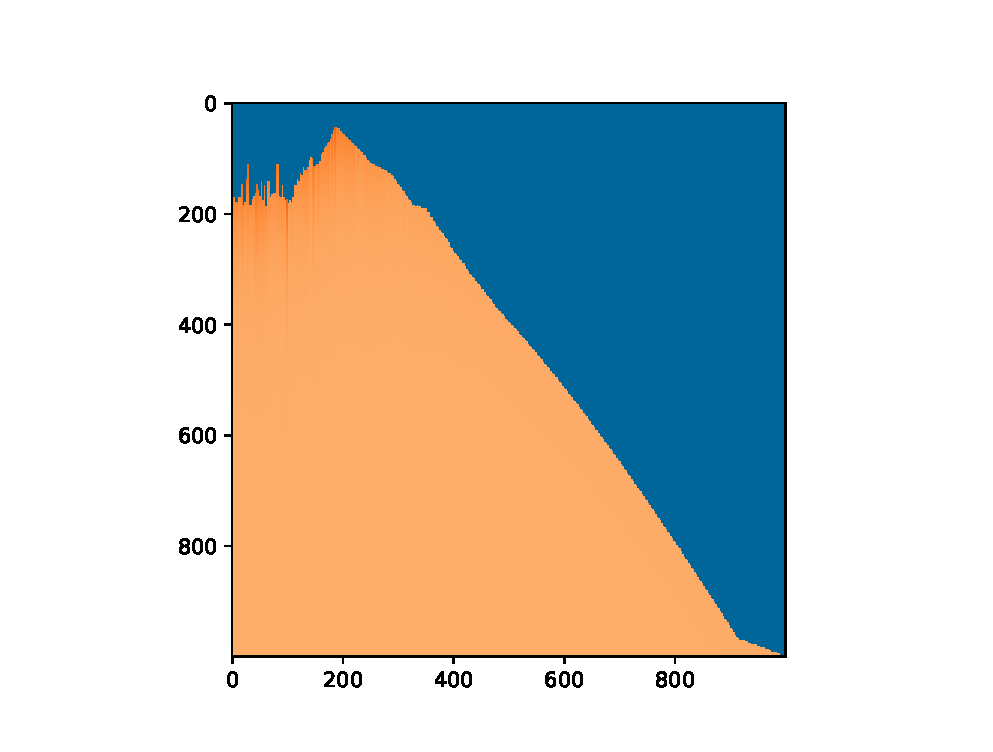
\includegraphics[width=\linewidth]{Figure_1.eps}
    \caption{A Windows Terminal.}
    \label{fig:Terminal}
\end{figure}

\section{Try Using BibTex}

This is a random citation \autocite{LeeRice-4} here.
% This is a random citation \cite{LeeRice-4} here.
And this would be another citation: \autocite{AragonRios-30}.
% And this would be another citation: \cite{AragonRios-30}.
Here's another \autocite{Starobin-32} one.
% Here's another \cite{Starobin-32} one.

\subsection{Footnote}
% If you use BibLaTex you may also use the default footnote of latex
Random citation \autocite{LeeRice-4} embedded in text.
This is some example text\footnote{\label{myfootnote}Hello footnote}.

\subsection{Refer to Footnote}
I'm referring to footnote \ref{myfootnote}.

\newpage
\begin{appendix}
    \listoffigures
    \listoftables
    \listoflistings
    % \bibliographystyle{ieeetr}
    \printbibliography
\end{appendix}
\end{document}
